\documentclass[12pt]{article}

\usepackage[margin=2cm]{geometry}
\usepackage[T2A]{fontenc}
\usepackage[utf8]{inputenc}
\usepackage[russian]{babel}
\usepackage{multicol}
\usepackage{longtable}
\usepackage{graphics}
\usepackage{rotating}
\usepackage{float}

\setlength{\parindent}{0em}
\setlength{\parskip}{1em}

\usepackage{amsmath, amsfonts, amssymb, amsthm, mathtools}
\usepackage{icomma}

\title{Отчет о выполнении лабораторной работы \\ Определение вязкости воздуха по скорости течения через тонкие трубки}
\author{Лепарский Роман}
\date{\today}

\begin{document}

\maketitle

\newpage

\section{Аннотация}

\textbf{Цель работы:} экспериментально исследовать свойства течения газов по тонким трубкам при различных числах Рейнольдса; выявить область применимости закона Пуазейля и с его помощью определить коэффициент вязкости воздуха.

\section{Теоретические сведения}

 В данной работе нам предлагается исследовать течение газа через тонкие трубки. Характер этого течения определяется числом Рейнольдса:
 \begin{equation}
 	Re = \frac{\rho u a}{\eta}
 	\label{eq:reinolds}
 \end{equation}
 
 Экспериментально установлено, что в рамках данного опыта критическое число Рейнольдса $Re_{\text{кр}}$ ниже которого поток можно считать ламинарным равно $10^3$
 
 Найдем характерные для этого течения величины. 
 
 \begin{figure}[H]
 	\centering
 	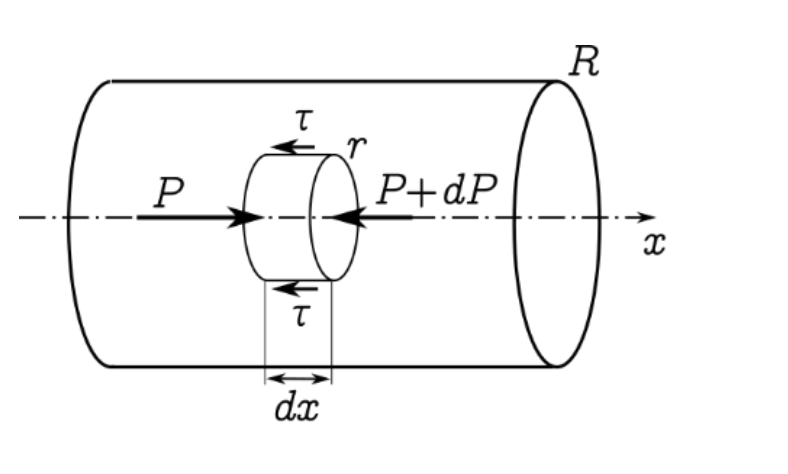
\includegraphics[scale = 0.3]{./images/puasel.png}
 	\label{fig:puasel}
 \end{figure}
 
 Для стационарного течения справедливо:
 
 \begin{align*}
 	F_{1x} &= -dP\cdot \pi r^2 \\
 	F_{2x} &= -\tau \cdot 2\pi r dx\\
 	\tau &= -\eta \frac{du}{dr}
 \end{align*}
 
 Из этих уравнений:
 \begin{equation}
	\frac{dp}{dx} = -\eta \frac{2}{r} \frac{du}{dr}
 \end{equation}
 
 Левая часть уравнения является градиентом давления, а правая не зависит от $x$. Поэтому справедливы следующие утверждения:
 
 \begin{align}
 	P(x) &= P_0 - \frac{\Delta P}{l}x \\
 	u(r) &= u_{max} - \frac{\Delta P}{4l}r^2
 \end{align}
 
 Если принять, что скорость газа вблизи стенок равна нулю, получим:
 \[
 	u(r) = \frac{\Delta P}{4l}(R^2 - r^2)
 \]
 
 Теперь можно получить формулу объемного расхода:
 \begin{equation}
 	Q = \int\limits_{0}^R u(r)\cdot 2\pi rdr = \frac{\pi R^4\Delta P}{8\eta l}
 	\label{eq:puasel}
 \end{equation}
 
 Формула Пуазейля (\ref{eq:puasel}) позволяет найти вязкость газа по зависимости расхода от перепада  давления в трубе и используется в качестве основной расчётной формулы в данной работе.
 
 Параболический профиль течения устанавливается не сразу, а только на некотором расстоянии $l_{\text{уст}} \approx 0,2R\cdot Re$
  \begin{figure}[H]
 	\centering
 	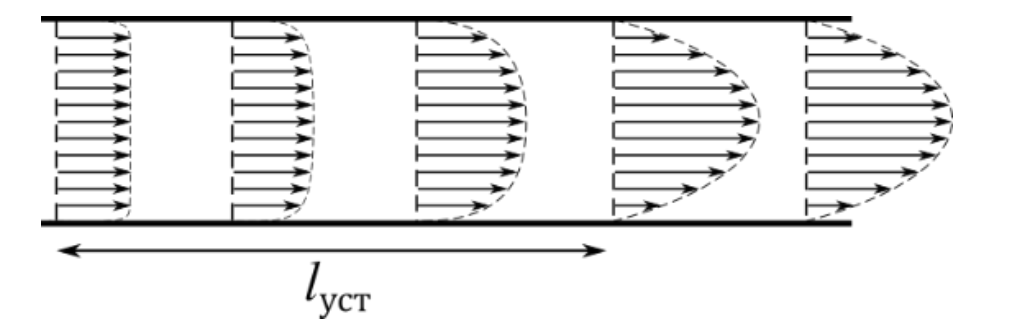
\includegraphics[scale = 0.2]{./images/lust.png}
 	\label{fig:lust}
 \end{figure}

Экспериментально длину установления можно определить, измеряя распределение давления вдоль трубки $P(x)$. На неустановившемся участке будет наблюдаться отклонение от линейного закона.

Коэффициент вязкости идеального газа можно описать следующей формулой:
\begin{equation}
	\eta \thicksim \frac{1}{3}\rho \bar{v}\lambda
\end{equation}

Для турбулентного течения в рамках некоторой теоретической модели можно получить соотношение 
\begin{equation}
	Q= \pi R^2 \bar{u} \thicksim R^{5/2} \sqrt{\frac{\Delta P}{\rho l}}
\end{equation}

\section{Экспериментальная установка}

\begin{figure}[H]
	\centering
	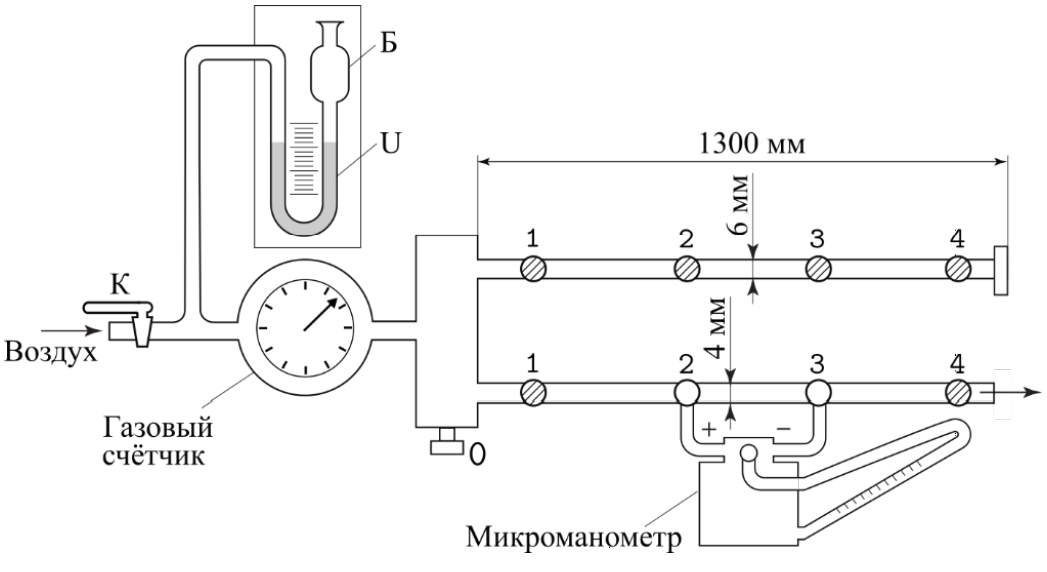
\includegraphics[scale = 0.4]{./images/stand.png}
	\caption{Схема установки}
	\label{fig:stand}
\end{figure}

Поток воздуха
под давлением, немного превышающим атмосферное, поступает через газовый счётчик в тонкие металлические трубки. Воздух нагнетается компрессором, интенсивность его подачи регулируется краном К. Трубки снабжены съёмными заглушками на концах и рядом миллиметровых отверстий, к которым можно подключать микроманометр. В рабочем состоянии открыта заглушка на одной (рабочей) трубке, микроманометр подключён к двум её выводам, а все остальные отверстия плотно закрыты пробками.

\section{Приборы и материалы}

В работе используются:

\begin{itemize}
	\item Система подачи воздуха;
	\item Газовый счетчик барабанного типа;
	\item Спиртовой микроманометр с регулируемым наклоном;
	\item Набор трубок различного диаметра с выходами для подсоединения микроманометра;
	\item Секундомер.
\end{itemize}

\section{Обработка результатов}

В данной работе нам предлагается исследовать течение воздуха через трубки разных диаметров. Измерим зависимость Расхода от давления. Примем $\sigma_{\Delta P} = 0,9$ Па, $\sigma_Q = 1,3\cdot10^{-4}$ л/с.


\begin{table}[H]
	\centering
	\begin{tabular}{|l|l|l|l|l|l|}
		\hline
		\multicolumn{2}{|l|}{d = 4 mm, l = 50 cm}                                & \multicolumn{2}{l|}{d = 3 mm, l = 20 cm}       & \multicolumn{2}{l|}{d = 5 mm, l = 90 cm}       \\ \hline
		 $\Delta P$, Pa & $Q$, l/s & $\Delta P$, Pa & $Q$, l/s & $\Delta P$, Pa & $Q$, l/s \\ \hline
		19,6                                                          & 0,0119   & 19,6                                & 0,0209   & 19,6                                & 0,0150   \\ \hline
		39,2                                                          & 0,0246   & 39,2                                & 0,0403   & 39,2                                & 0,0377   \\ \hline
		58,8                                                          & 0,0384   & 58,8                                & 0,0556   & 58,8                                & 0,0556   \\ \hline
		78,4                                                          & 0,0512   & 78,4                                & 0,0675   & 78,4                                & 0,0752   \\ \hline
		98,0                                                          & 0,0625   & 98,0                                & 0,0781   & 98,0                                & 0,0967   \\ \hline
		117,6                                                         & 0,0757   & 117,6                               & 0,0886   & 117,6                               & 0,1091   \\ \hline
		137,2                                                         & 0,0877   & 137,2                               & 0,0972   & 137,2                               & 0,1154   \\ \hline
		156,8                                                         & 0,0925   & 196,0                               & 0,1167   & 196,0                               & 0,1428   \\ \hline
		196,0                                                         & 0,0996   & 235,2                               & 0,1269   & 235,2                               & 0,1581   \\ \hline
		235,2                                                         & 0,1063   & 274,4                               & 0,1363   & 274,4                               & 0,1638   \\ \hline
		274,4                                                         & 0,1129   & 313,6                               & 0,1454   &                                     &          \\ \hline
		313,6                                                         & 0,1201   & 352,8                               & 0,1556   &                                     &          \\ \hline
		352,8                                                         & 0,1246   & 392,0                               & 0,1627   &                                     &          \\ \hline
		392,0                                                         & 0,1333   & 431,2                               & 0,1682   &                                     &          \\ \hline
		431,2                                                         & 0,1404   &                                     &          &                                     &          \\ \hline
	\end{tabular}
\end{table}

Построим графики и найдем коэффициент наклона в ламинарной области.
\begin{figure}[H]
	\centering
	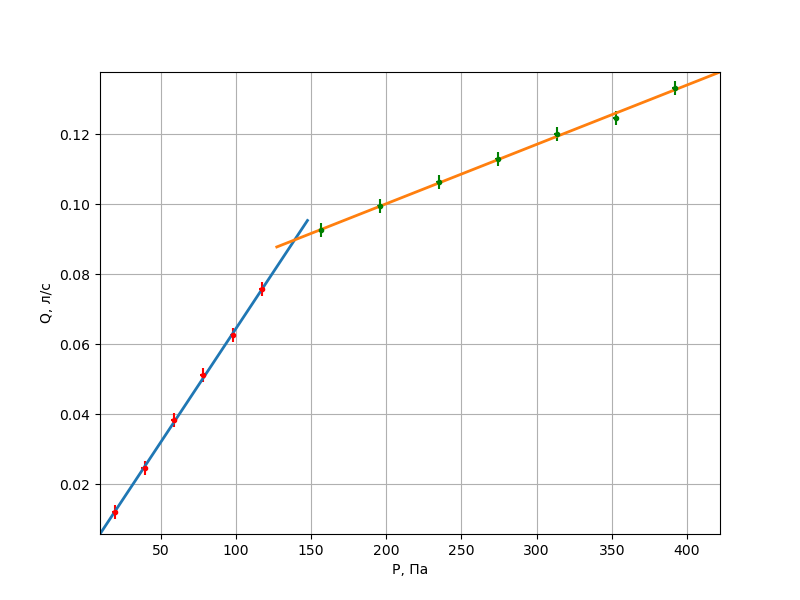
\includegraphics[scale=0.55]{./images/d4mm1.png}
	\caption{$k = (649\pm6)\cdot 10^{-6}$ л/с$\cdot$Па}
\end{figure}

Из формулы (5) найдем вязкость $\eta = (1,81\pm 0,05)*10^{-5}$ кг$\cdot$м/с. А по формуле $Re = \frac{QR\rho}{S\eta}$
Найдем $Re_{kr} = 964\pm9$

Проделаем то же самое для других диаметров. $d = 3$ мм:
\begin{figure}[H]
	\centering
	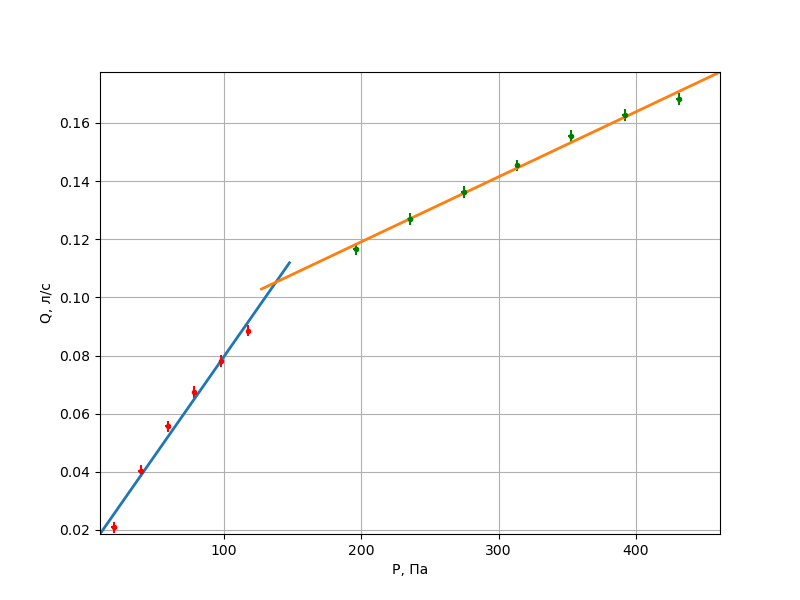
\includegraphics[scale=0.55]{./images/d3mm1.png}
	\caption{$k = (67\pm3)\cdot 10^{-5}$ л/с$\cdot$Па}
\end{figure}
$\eta = (1,4\pm 0,2)*10^{-5}$ кг$\cdot$м/с, $Re_{kr} = 1010\pm12$

Для $d = 5$ мм:
\begin{figure}[H]
	\centering
	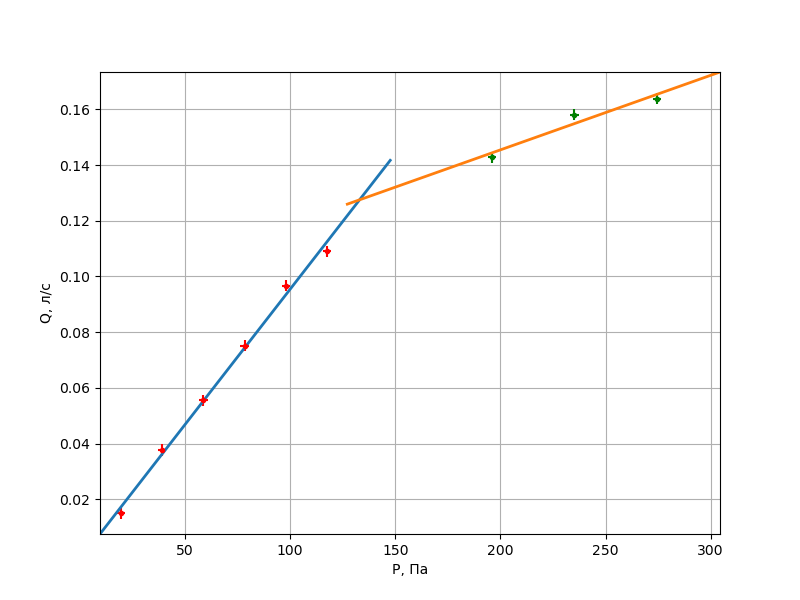
\includegraphics[scale=0.55]{./images/d5mm1.png}
	\caption{$k = (97\pm2)\cdot 10^{-5}$ л/с$\cdot$Па}
\end{figure}

$\eta = (1,75\pm 0,17)*10^{-5}$ кг$\cdot$м/с, $Re_{kr} = 1108\pm19$

Теперь попробуем определить длину установления.
\begin{figure}[H]
	\centering
	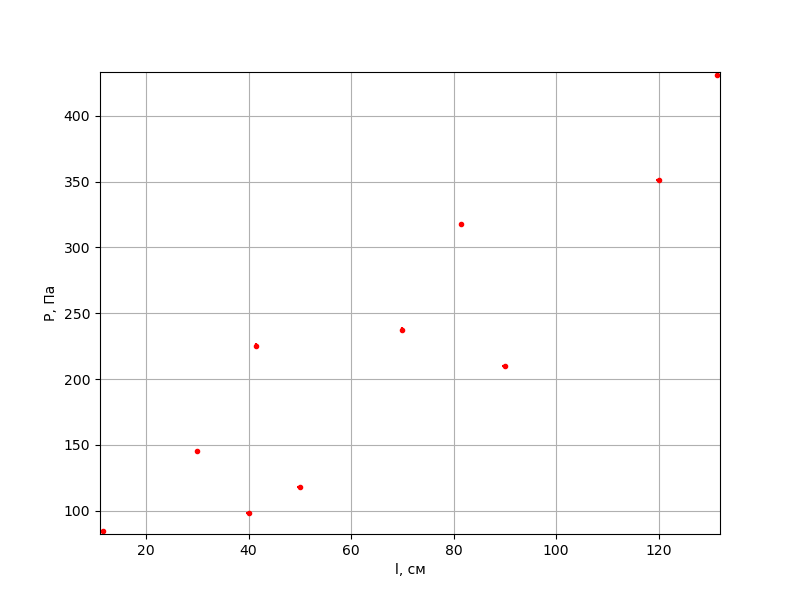
\includegraphics[scale=0.55]{./images/d4mm2.png}
	\caption{$d = 4$ мм}
\end{figure}
\begin{figure}[H]
	\centering
	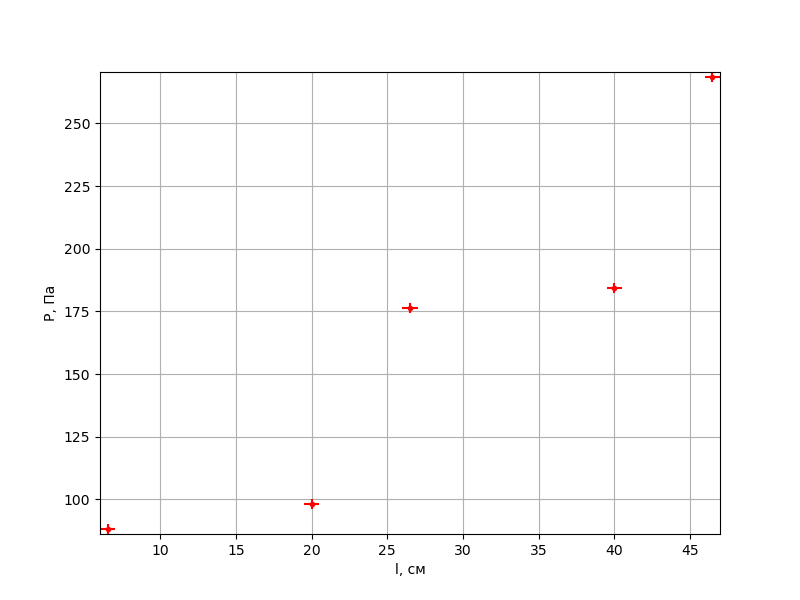
\includegraphics[scale=0.55]{./images/d3mm2.png}
	\caption{$d = 3$ мм}
\end{figure}
\begin{figure}[H]
	\centering
	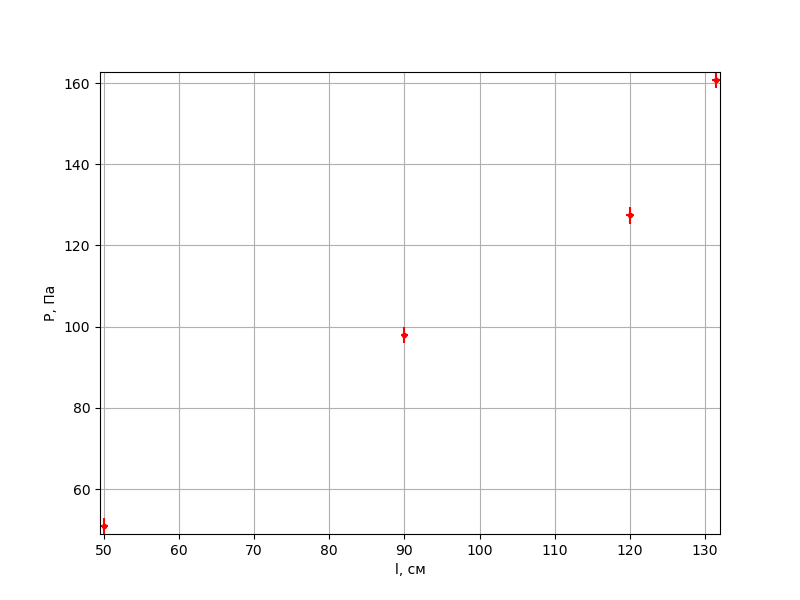
\includegraphics[scale=0.55]{./images/d5mm2.png}
	\caption{$d = 3$ мм}
\end{figure}

Из этих графиков не получается найти длину установления.


\section{Вывод}

Нам удалось исследовать течение газа через тонкие трубки. Мы выявили границы применимости закона Пуазейля. С помощью этого закона мы нашли вязкость воздуха $\eta = 1,65\pm0.11$ кг$\cdot$м/с и критическое число Рейнольдса  $Re_{kr} = 1027\pm30$. Полученные результаты схожи с табличными: $\eta = 1,78$ кг$\cdot$м/с, $Re_{kr} = 1000$. К сожалению, не удалось найти длину установления. Причиной этого может быть положение крайнего вентиля.


\end{document}